\documentclass{article}

\textwidth=6.5in
\textheight=8.5in
\voffset=-54pt
\oddsidemargin=0in
\evensidemargin=0in
\setlength{\parskip}{8pt}
\setlength{\parindent}{0pt}

\usepackage{amsmath, amssymb}
\usepackage{ifthen}

\usepackage[inline]{enumitem}
\setlist{topsep=0pt, parsep=8pt}

\usepackage[rgb,table]{xcolor}\convertcolorsUfalse
\usepackage{graphicx}

% change hyperref options
\PassOptionsToPackage{hyphens}{url}
\usepackage[bookmarks,colorlinks,linkcolor=black,citecolor=blue,pdfstartview=FitH,urlcolor=blue]{hyperref}
\hypersetup{pdfpagemode=UseNone}
\usepackage{bookmark}

\usepackage{graphicx}
\usepackage{multicol}
\usepackage{framed}
\usepackage{array}

\usepackage{icomma}

\usepackage{pifont}

\usepackage{marginnote}
\usepackage[colorinlistoftodos]{todonotes}
\renewcommand{\marginpar}{\marginnote}

\usepackage{soul}

\usepackage{pgfplots}
\pgfplotsset{compat=1.18}  
\pgfplotscreateplotcyclelist{mycolor}{black, blue, red, green!70!black, magenta, purple, cyan, orange }  
\pgfplotsset{
  disabledatascaling,
  cycle list=tikzcolor, 
  axis lines=middle,
  every axis plot/.style={no marks, thick},
  every axis/.style={
    enlarge x limits=false,
    enlarge y limits=auto,
    xlabel style={at={(current axis.right of origin)},anchor=west},
    ylabel style={at={(current axis.above origin)},anchor=south},
    % extra x and y ticks for asymptotes
    extra x tick style={grid=major, grid style={dashed,black}},
    extra y tick style={grid=major, grid style={dashed,black}},
    /pgf/number format/1000 sep={},
  },    
  tick label style = {font=\footnotesize, fill=\currentbgcolor, inner sep=0pt},    
  xticklabel shift=1pt,    
  scaled ticks=false,
  scaled y ticks=false,
  unbounded coords=jump,
  samples=101,
  minor tick length=0,
  scatter/classes={
    open={mark=*,draw=black,fill=white, mark size=2, thin},
    closed={mark=*,draw=black,fill=black, mark size=2, thin}
  },
  width=3in,
}
\pgfplotsset{open/.style={only marks, mark=*, fill=white, thin, mark size=2}}
\pgfplotsset{closed/.style={only marks, mark=*, draw=black, fill=black,
    thin, mark size=2}}
\pgfplotsset{labeled/.style={nodes near coords, only marks, mark=*, draw=black, fill=black, thin, mark size=2, point meta=explicit symbolic}}

\pgfplotsset{gridgraph/.style={clip=false, axis line style={shorten
      >=-8pt}, xlabel style={xshift=8pt}, ylabel style={yshift=8pt},
    enlargelimits=false, grid=major, tick style={black}}} 

\usepackage{tikz}
\usetikzlibrary{
  matrix,%
  % enables the snake paths
  decorations.pathmorphing,%
  % enables bigger arrows
  decorations.markings,%
  decorations.pathreplacing,%
  decorations.text,%
  calc,%
  patterns,%
  shapes.geometric,%
  arrows,
  decorations.shapes,
  positioning,
  plotmarks,
  intersections
}
\tikzset{>=latex} % sets default arrow type in tikz
\tikzset{font=\normalsize}
\tikzset{mark size=1.5pt, mark options=thin}
\tikzset{pin distance=4pt,
  every pin edge/.style={<-, thin, shorten <= -2pt}}

\interfootnotelinepenalty=10000
\renewcommand{\thefootnote}{(\arabic{footnote})}

\usepackage{multirow, bigdelim}

% change to \usepackage[sols]{handout} to see solutions
\usepackage[]{handout}

\providecommand{\check}{}
\renewcommand{\check}{\ifmmode{\text{ \ding{51} }}\else{\ding{51} }\fi}

\newcommand\iscurrentenumi[1]{%
  \ifthenelse{\equal{#1}{\theenumi}}{}{#1}}
\setenumerate[1]{ref=\#\arabic*}
\setenumerate[2]{ref=\protect\iscurrentenumi{\theenumi}(\alph*)}
\newcommand\enumiiprefix[2]{%
  \ifthenelse{{\equal{#1}{\theenumi}}\AND{\equal{#2}{(\alph{enumii})}}}{}{}%
  \ifthenelse{{\equal{#1}{\theenumi}}\AND{\NOT{\equal{#2}{(\alph{enumii})}}}}{#2}{}%
  \ifthenelse{\equal{#1}{\theenumi}}{}{#1#2}%
}
\setenumerate[3]{ref=\protect\enumiiprefix{\theenumi}{(\alph{enumii})}\roman*}

\makeatletter

% underline links               
\let\@href=\href
\renewcommand{\href}[2]{\@href{#1}{\ul{#2}}}

\newdimen\SOUL@dimen %new
\def\SOUL@ulunderline#1{{%
    \setbox\z@\hbox{#1}%
    % \dimen@=\wd\z@
    \SOUL@dimen=\wd\z@ %new
    \dimen@i=\SOUL@uloverlap
    \advance\SOUL@dimen2\dimen@i %\dimen@ exchanged too
    \rlap{%
      \null
      \kern-\dimen@i
      % \SOUL@ulcolor{\SOUL@ulleaders\hskip\dimen@}%
      \SOUL@ulcolor{\SOUL@ulleaders\hskip\SOUL@dimen}% new
    }%
    \unhcopy\z@
  }}

\makeatother

\renewcommand{\answer}[1]{#1}

\definecolor{purple}{rgb}{0.5,0,1.0}
\definecolor{skyblue}{rgb}{0, 0.5, 1}

\newcommand{\highlight}[1]{\boldmath\hl{\textbf{#1}}\unboldmath}

\newcommand{\goal}[1]{\textbf{\textcolor{skyblue}{#1}}}

\usepackage{fancyhdr}
\lhead{\textcolor{white}{This content is protected and may not be shared, uploaded, or distributed.}}
\rhead{}
\rfoot{\vspace*{\fill}\footnotesize\textcopyright{} \emph{Harvard Math Ma}}
\renewcommand{\headrulewidth}{0pt}
\pagestyle{fancy}
\begin{document}

\htitle{27. Exam 2 Practice}
\emph{These are review problems, not meant to be exhaustive, but to return to topics from a few weeks ago. Work on these or practice exam questions during your section today.}
\begin{enumerate}
\item  \emph{You be the grader!}

  \begin{enumerate}
  \item
    \begin{problem}[0.25in]
      A Math Ma student is working on the following problem.
      \begin{quote}
        Sketch an example of a function $f(x)$ such that $\displaystyle
        \lim_{x \to 2^-} f(x)$ and $\displaystyle \lim_{x \to 2^+}
        f(x)$ both exist but $\displaystyle \lim_{x \to 2} f(x)$ does not
        exist. 
      \end{quote}
      The student submits the answer below. What feedback would you give them?

      \begin{tikzpicture}
        \begin{axis}[xtick={2}, ytick=\empty, extra x ticks={2}, enlarge
          y limits=false, width=1.75in, height=1.75in]
          \addplot+[domain=-1:5] {1/(x-2)};
        \end{axis}
      \end{tikzpicture}
    \end{problem}

    \begin{solution}
      Here's an example of possible feedback.

      It's true that, for the function $f(x)$ you sketched, 
      $\lim\limits_{x \to 2} f(x)$ does not exist. However, the one-sided
      limits also do not exist. For your function, 
      $\lim\limits_{x \to 2^-} f(x) = -\infty$
      and $\lim\limits_{x \to 2^+} f(x) = \infty$. Remember that
      when we say that a limit is ``equal'' to $\pm \infty$, it is shorthand
      for ``the limit does not exist because the function is
      increasing/decreasing without bound.''

      Here's an example of a correct response.
      
      \begin{tikzpicture}
        \begin{axis}[xtick={2}, ytick=\empty, width=1.75in, height=1.75in]
          \addplot+[domain=-1:2] {1};
          \addplot[domain=2:5] {-1};
          \addplot[open] coordinates {(2, 1) (2, -1)};
        \end{axis}
      \end{tikzpicture}
      
    \end{solution}

  \item
    \begin{problem}[\vfill\newpage]
      Another student is working on this problem.
      \begin{quote}
        Given the graphs of $f$ and $g$ below, find $\displaystyle \lim_{x \to 2} f(x) g(x)$ and $\displaystyle \lim_{x \to 1} \frac{f(x)}{g(x)}$.
        \begin{center}
          \begin{tikzpicture}
            \begin{axis}[gridgraph, axis equal image, title=$f$, ymin=-2,
              ymax=2, width=2.5in] 
              \addplot+[domain=0:2] {x-1};
              \addplot+[domain=2:4] {x - 3};
              \addplot+[open] coordinates { (2, 1) };
              \addplot+[closed] coordinates { (2, -1) };
            \end{axis}
          \end{tikzpicture}
          \hspace{0.5in}
          \begin{tikzpicture}
            \begin{axis}[gridgraph, axis equal image, title=$g$, ymin=-2, width=2.5in]
              \addplot+[domain=0:2] {2-2*x};
              \addplot+[domain=2:4] {2};
              \addplot+[open] coordinates { (2, 2)  (2,  -2)};
              \addplot+[closed] coordinates { (2, -1) };
            \end{axis}
          \end{tikzpicture}          
        \end{center}
      \end{quote}
      The student writes:
      \begin{quote}
        Since $\displaystyle \lim_{x \to 2} f(x)$ DNE, $\displaystyle \lim_{x \to 2} f(x) g(x)$ DNE. Since $\displaystyle \lim_{x \to 1} f(x) = 0$, $\displaystyle \lim_{x \to 1} \frac{f(x)}{g(x)} = 0$.
      \end{quote}
      What feedback would you give the student?
    \end{problem}

    \begin{solution}
      Here's an example of possible feedback.

      If $\lim\limits_{x\to 2} f(x)$ and $\lim\limits_{x\to 2} g(x)$
      existed, then $\lim\limits_{x\to 2} f(x)g(x)$ would have been the product
      of the two limits:
      \[\lim_{x \to 2} f(x)g(x) = \left[\lim_{x \to 2}f(x)\right] \cdot
      \left[\lim_{x \to 2} g(x) \right]
      \]
      However, as $x$ approaches $2$, neither $f(x)$ nor $g(x)$ approach a
      particular value. \textbf{This does not mean that the product
      $f(x)g(x)$ will
      not approach a particular value.}

      Similarly, if $\lim\limits_{x \to 1} g(x)$ was not zero, 
      then $\lim\limits_{x \to 1} \dfrac{f(x)}{g(x)}$ would have been the quotient
      of the two limits:
      \[\lim_{x \to 1} \frac{f(x)}{g(x)} = \frac{\lim\limits_{x \to 1} f(x)}
      {\lim\limits_{x \to 1} g(x)}\]
      As $x$ approaches $1$, $f(x)$ approaches $0$ but $g(x)$ also approaches $0$,
      so \textbf{the individual limits don't tell us what value, 
      if any, $f(x)/g(x)$ approaches.}

      Here's an example of a correct response.

      Since $\lim\limits_{x \to 2} f(x)$ and $\lim\limits_{x \to 2} g(x)$ do not exist, 
      let's inspect their one-sided limits. As $x$ approaches $2$ from the left,
      $f(x)$ approaches $1$ and $g(x)$ approaches $-2$, so 
      $\lim\limits_{x \to 2^-} f(x)g(x) = -2$. As $x$ approaches $2$ from the right,
      $f(x)$ approaches $-1$ and $g(x)$ approaches $2$, so 
      $\lim\limits_{x \to 2^+} f(x)g(x) = -2$. Since the one-sided limits are equal,
      $\lim\limits_{x \to 2} f(x)g(x) = -2$.

      Since $\lim\limits_{x \to 0} f(x)$ and $\lim\limits_{x \to 0} g(x)$ are both zero,
      we should try to factor and cancel. Around $x=1$, $f(x)=x-1$ and $g(x) = -2x+2$.
      \begin{align*}
        \lim_{x \to 1} \frac{f(x)}{g(x)} &= \lim_{x \to 1} \frac{x-1}{-2x+2} \\
        &= \lim_{x \to 1} \frac{x-1}{-2(x-1)} \\
        &= -\frac{1}{2}
      \end{align*}
      
    \end{solution}
  \end{enumerate}

\item  % 10.3.18

  \begin{problem}[\newpage]
    Q-Tips$^{\text{\textregistered}}$ are a brand of 3-inch long cotton swabs. The manufacturer would like to sell them in boxes with volume 37.5 cubic inches. One side of the box is made from cardboard, and the other five sides are made of plastic; to fit the swabs, one edge of the cardboard must be 3 inches long. What dimensions should the box be to minimize the amount of plastic used?
  \end{problem}  

  \begin{solution}
    \highlight{Goal: } Minimize the amount of plastic used.

    \highlight{Define variables:}
    The box looks roughly like the picture below, where the blue is plastic and the brown is cardboard. We are given one dimension (the width).
    \begin{center}
      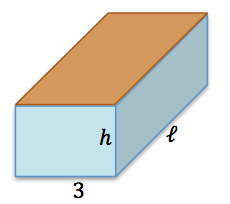
\includegraphics[width=100px]{images/qtips.png}
    \end{center}
    
    \highlight{Formula for goal:}
    The amount of plastic is equal to the area of the 5 plastic sides,
    \[P=2(3h)+3\ell=6h+3\ell+2h\ell\]
    To get a function of one variable, we need to \highlight{relate the variables
    using information from the problem.} We're told that the volume of the box
    is $37.5$ cubic inches, so
    \begin{align*}
      3hl &= 37.5 \\
      h &= \tfrac{37.5}{3\ell} \\
      &= \tfrac{12.5}{\ell}
    \end{align*}
    Substituting this back into our formula for the area, we get the function
    \[P(\ell) = 6[\tfrac{12.5}{\ell}+3\ell+2\ell(\tfrac{12.5}{\ell})]=
    \tfrac{75}{\ell}+3\ell+25\]
    We can see that the length can get pretty much as small as we want it to be (as long
    as it is wider than one Q-Tip), and we can make the length arbitrarily large
    by making $h$ as small as we want. So the domain of the function is $\ell > 0$,
    or $(0, \infty)$.  
    
    \highlight{Critical points:}
    First, we use derivative rules to determine that $P'(\ell)=-\frac{75}{\ell^2}+3$.
    $P'(\ell)$ is undefined when $\ell=0$, but this is not in the domain. 
    \begin{align*}
      -\tfrac{75}{\ell^2} + 3 &= 0 \\
      \tfrac{75}{\ell^2} &= 3 \\
      \ell^2 &= 25 \\
      \ell &= \pm 5
    \end{align*}
    There are two solutions when we set $P'(\ell)=0$ and solve for $\ell$, 
    but $\ell=-5$ is not in the domain,
    so the only critical point is $\ell=5$.

    \highlight{Global minimum: }
    Since there is only one critical point, if we can show that it is a local minimum,
    then it will show that it is the global minimum. Let's use the Second Derivative Test.
    $P''(\ell)=\frac{150}{\ell^3}$, which is indeed positive for $\ell=5$, so the global
    minimum occurs at $\ell = 5$.
    
    \highlight{Answer the question:} Finally, we find $h=\frac{12.5}{5}=2.5$. So, the
    dimensions of the box that minimize the amount of plastic are 
    \fbox{$l=5$ inches and $h=2.5$ inches}.
  \end{solution}

  % \item ({\it 10.3.11}) % 10.3.11
  %   \label{probDRG-14}%
  %   Below is a graph of $f'(x)$. The questions that follow are questions
  %   about~$f$.
  %   \begin{center}
  %     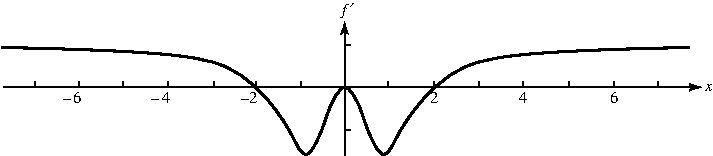
\includegraphics{art/go10p11}
  %   \end{center}
  %   
  %   \begin{enumerate}
  %     
  %   \item Identify all critical points of $f$.  Are these critical points
  %     also stationary points? (\emph{Recall:} A stationary point is a point
  %     at which $f'=0$.)
  %     
  %     
  %   \item On a number line plot all the critical points of $f$. Use the
  %     number line to indicate the sign of $f'$; above this indicate where
  %     the graph of $f$ is increasing and where it is decreasing.
  %     
  %     \begin{enumerate}
  %     \item graph of $f$ \underline{\hspace{20pc}}
  %       
  %     \item sign of $f'$
  %     \end{enumerate}
  %     
  %     
  %   \item Some of the $x$-intercepts of $f'$ correspond to the local extrema
  %     of $f$. How can you determine which ones do?
  %   \item On a number line plot all the critical points of $f'$. Use the
  %     number line to indicate the sign of $f''$; above this indicate where
  %     the graph of $f$ is concave up and where it is concave down.
  %     
  %     \begin{enumerate}
  %       
  %     \item graph of $f$ \underline{\hspace{20pc}}
  %       
  %     \item sign of $f''$
  %     \end{enumerate}
  %     
  %     
  %     
  %   \item Explain why the local extrema of $f'$ correspond to the points of
  %     inflection of $f$.
  %   \item Suppose $f(0) = 0$. Draw a rough sketch of the graph of~$f$.
  %     
  %   \end{enumerate}

\item 

  \emph{E.~coli} is a bacteria sometimes found in ground beef that can cause fatal food poisoning. Naturally, food safety inspectors would like to be able to test for it; the challenge is to be able to take a tiny sample of ground beef (so that the rest can be sold to customers) and check for \emph{E.~coli}, even if the sample has just a single bacterium.

  % "For lethal threats, like \emph{E.~coli} O157 in ground beef, the
  % detection process involves a grim recipe of ground beef and a
  % broth infused with nutrients that \emph{E.~coli} likes to eat, put in a
  % warm place to rest for 10 hours — at which point a single \emph{E.~coli}
  % cell, if it exists, will have spawned one million easy-to-detect
  % siblings."

  DNA tests aren't sensitive enough to detect just a single bacterium, so food inspectors \href{https://people.math.harvard.edu/~jjchen/mathma/docs/articles/private-eyes-in-the-grocery-aisles.html}{put the ground beef sample in ``a broth infused with nutrients that \emph{E.~coli} likes to eat\ldots to rest for 10 hours''}. Let's understand why. Under such conditions, it's estimated that a population of \emph{E.~coli} doubles every 30 minutes.

  \begin{enumerate}

  \item

    \begin{problem}[\vfill]
      How many \emph{E.~coli} are there $t$ minutes after a single bacterium is put in the broth?
    \end{problem}

    \begin{solution}

      \begin{tabular} {l| l }
        $t$ & \begin{tabular} {l} $\#$ of bacteria\\  after $t$ minutes\end{tabular} \\ 
        \hline 
        0 & 1 \\ 
        30 & 2 \\ 
        60 & 4 \\ 
        90 & 8 
      \end{tabular}

       \fbox{$B = 2^{t/30}$}
    \end{solution} 

  \item

    \begin{problem}[\vfill]
      How many \emph{E.~coli} are there $h$ hours after a single bacterium is put in the broth?
    \end{problem}

    \begin{solution}
      Since $t=60h$, plugging this 
      into $B=2^{t/30}$ gives \fbox{$B = 2^{2h}$}.
    \end{solution}

  \item

    \begin{problem}[\stretch{0.25}]
      \check What kind of check can you do to make sure your answers are reasonable?
    \end{problem}

    \begin{solution}
      We can plug in some values of $t$ and $h$ and check if we get the expected outputs.
    \end{solution}

  \item
    \begin{problem}[0.25in]
      How many bacteria are there after 10 hours? Use the fact that $2^{10} \approx 1000$ to estimate roughly how big this number is.
    \end{problem}

    \begin{solution} 
      When $h=10$, $B=2^{20}$. 
      This is $(2^{10})^2 \approx 1000^2$, or about $1,000,000$. 
    \end{solution}

  \item
    \begin{problem}[\nstretch{0.25}]
      By what percent does the number of bacteria in the broth grow per hour?
    \end{problem}

    \begin{solution}
      We can rewrite $B=2^{2h}$ as $B=(2^2)^h=4^h$. This shows that the number
      of bacteria quadruples every hour, which is a \fbox{$300\%$} increase.
    \end{solution}

  \end{enumerate}

\item  %\points{19} 

  Let $g(x) = x^3 - 12x$. 

  \begin{enumerate}

  \item
    \begin{problem}[\stretch{0.4}]
      Is $g$ even, odd, or neither? Justify your answer. 
    \end{problem}

    \begin{solution}
      To answer this, we look at $g(-x)$:
      \begin{align*}
        g(-x) &= (-x)^3 - 12 (-x) \\
        &= - x^3 + 12 x \\
        &= - g(x),
      \end{align*}
      so $g$ is \fbox{odd}. 
    \end{solution}

  \item
    \begin{problem}[\vfill]
      Find all critical points of $g$, and classify each as a local minimum, local maximum, or neither. 
    \end{problem}

    \begin{solution} 
      To answer this, we'll make a sign chart for $g'(x) = 3x^2 - 12$. First, $g'$ is never undefined, and $g'(x) = 0$ when $x = \pm 2$. Testing points gives us the following sign chart:
      \begin{center}
        \begin{tikzpicture}
          \begin{axis}[axis y line=none, x axis line style={-}, xtick={-2, 2}, ymin=-2, ymax=2, height=1.25in, width=3in, clip=false]
            \addplot+[domain=-10:6, very thin]{0};
            \draw(-10, 0) node[anchor=south west] {$g$};%
            \draw (-10, -1.5) node[right] {sign of $g'$};%
            \draw (-4, -1.5) node{$+$};%
            \draw[->, xshift=2pt] (-5.6, 0.5) -- (-2.4, 1.5);%
            \draw (0, -1.5) node{$-$};%
            \draw[->, xshift=2pt] (-1.6, 1.5) -- (1.6, 0.5);%
            \draw (4, -1.5) node{$+$};%
            \draw[->, xshift=2pt] (2.4, 0.5) -- (5.6, 1.5);%
            \draw[->, xshift=2pt] (-2.4, 1.5) -- (-1.6, 1.5);%
            \draw[->, xshift=2pt] (1.6, 0.5) -- (2.4, 0.5);%
          \end{axis}
        \end{tikzpicture}        
      \end{center}
      So $g$ has two critical points: \fbox{a local maximum at $x=-2$
      and a local minimum at $x=2$}.
    \end{solution}

  \item

    \begin{problem}[\stretch{0.5}]
      What's the $y$-intercept of $g$? Is it easy to find the $x$-intercepts? If so, find them.
    \end{problem}

    \begin{solution}
      \answer{The $y$-intercept is $g(0) = 0$.} To find the $x$-intercepts, we solve
      \begin{align*}
        x^3 - 12 x &= 0 \\
        x (x^2 - 12) &= 0 
      \end{align*}
      So, $x = 0$ or $x = \pm \sqrt{12} = \pm 2 \sqrt{3}$. That is, \fbox{the $x$-intercepts are $x = 0, \pm 2 \sqrt{3}$}. 
    \end{solution}

  \item
    \begin{problem}[\nstretch{0.8}]
      Sketch a rough graph of $g(x)$. You need not depict the concavity accurately.
    \end{problem}

    \begin{solution}
      Since $g$ is odd, we can focus on graphing it on $[0, \infty)$ and then use symmetry to get the other half. We know $g(0) = 0$, $g$ is decreasing and concave up on $(0, 2)$, $g$ is increasing and concave up on $(2, \infty)$, and $g(2 \sqrt{3}) = 0$. So, that gives us something like this:
      \begin{center}
        \begin{tikzpicture}
          \begin{axis}[xtick={3.4641, 2}, xticklabels={$2\sqrt{3}$, $2$}, ytick=\empty]
            \addplot+[domain=-4.5:4.5, opacity=0] {x^3-12*x}; 
            \addplot+[domain=0:4.5] {x^3-12*x}; 
          \end{axis}
        \end{tikzpicture}
      \end{center}
      Then, since $g$ is odd, the entire graph looks like this:
      \begin{center}
        \answer{
          \begin{tikzpicture}
            \begin{axis}[xtick={-3.4641, 3.4641, -2, 2}, xticklabels={$-2\sqrt{3}$, $2\sqrt{3}$, $-2$, $2$}, ytick=\empty]
              \addplot+[domain=-4.5:4.5] {x^3-12*x}; 
            \end{axis}
          \end{tikzpicture}
        }
      \end{center}
    \end{solution}

  \end{enumerate}
  Let $f(x) = |g(2x)|$.
  \begin{enumerate}[resume]
  \item
    \begin{problem}[\stretch{0.75}]
      Sketch a rough graph of $f(x)$. Label any intercepts. 
    \end{problem}

    \begin{solution}
      The graph of $g(2x)$ is the graph of $g(x)$ stretched horizontally by a factor of $\dfrac{1}{2}$, so the graph of $f(x) = |g(2x)|$ looks like this:
      \begin{center}
        \answer{
          \begin{tikzpicture}
            \begin{axis}[xtick={-1.732, 1.732, -1, 1}, xticklabels={$-\sqrt{3}$, $\sqrt{3}$, $-1$, $1$}, ytick=\empty, xmin=-4.5, xmax=4.5]
              \addplot+[domain=-2.25:2.25, samples=260] {abs((2*x)^3-24*x)};
            \end{axis}
          \end{tikzpicture}
        }
      \end{center}
    \end{solution}

  \item
    \begin{problem}[\stretch{0.25}]
      Where (at what $x$-values) are the local minima of $f$? Where are the local maxima?
    \end{problem}

    \begin{solution}      
      From the graph, we can see the local minima are at $\boxed{x = \pm \sqrt{3}, 0}$ and the local maxima are at $\boxed{x = \pm 1}$. 
    \end{solution}

  \item
    \begin{problem}[\stretch{0.75}]
      Find the global maximum and minimum of $f$ on $[-2, 2]$. Please tell us both the global maximum / minimum value (the $y$-value) and where (at what $x$-value(s)) each occurs.
    \end{problem}

    \begin{solution}
      We can see from the graph that the global minimum on $[-2, 2]$ occurs
      at \fbox{$x=\pm\sqrt{3}$} and \fbox{$x=0$}, and the minimum value is \fbox{$y=0$}.

      Based on our graph, the global maximum could occur at at $x=\pm1$ or at the endpoints,
      $x=\pm2$. We need to compare the $y$-values at these points by plugging in the $x$-values
      to $f(x)$. We'll just find $f(1)$ and $f(2)$. Since $f$ is even, 
      we know $f(-1)=f(1)$ and $f(-2)=f(2)$. 
      \begin{align*}
        f(1) &= |g(2)| = |(2)^3-12(2)|= 16 \\
        f(2) &= |g(4)| = |(4)^3-12(4)| = 16
      \end{align*}
      Since all of these $y$-values are equal,
      the global maximum is attained at \fbox{$x=\pm1$ and
      $x=\pm2$}, and the maximum value is \fbox{$y=16$}.
    \end{solution}

  \end{enumerate}

\item 

  \begin{problem}[\vfill\newpage]
    Let $g(x) = 2^{x - 3} \cdot 5^{-x/2}$. Rewrite $g(x)$ in the form $g(x) = C \cdot b^x$, and sketch its graph. Label all intercepts and asymptotes. 
  \end{problem}

  \begin{solution}
    Using properties of exponents, we can rewrite $g(x)$.
    \begin{align*}
      g(x) &= 2^{x-3}\cdot 5^{-x/2} \\
      &= 2^{-3}(2^x \cdot 5^{-x/2}) \\
      &= \tfrac{1}{8}(2 \cdot 5^{-1/2})^x \\
      &= \tfrac{1}{8}(\tfrac{2}{\sqrt{5}})^x
    \end{align*}
    The graph of $y=g(x)$ is decreasing, has a horizontal asymptote at $y=0$, and
    the $y$-intercept is at $y=\frac{1}{8}$. There are no $x$-intercepts.
    \begin{center}
      \begin{tikzpicture}
        \begin{axis}[xtick=\empty, ytick={0.125}, yticklabels={$\frac{1}{8}$}]
          \addplot[domain=-15:15] {0.894427191^x/8};
        \end{axis}
      \end{tikzpicture}
    \end{center}
  \end{solution}

\item 

  Here's the graph of the function $f$ and a formula for a function $g$.

  \begin{multicols}{2}
    \begin{tikzpicture}
      \begin{axis}[gridgraph, axis equal image, xtick={-3, ..., 3}]
        \addplot+[domain=-1:1] {1 - x^2}; %
        \addplot+[sharp plot] coordinates { (-3, 1) (-1, -1) }; %
        \addplot+[sharp plot] coordinates { (1, -2) (3, 2) }; %
        \addplot+[closed] coordinates {(-3, 1) (-1, -1) (1, 1) (3, 2)};%
        \addplot+[open] coordinates {(-1, 0) (1, 0) (1, -2)}; %
      \end{axis}
    \end{tikzpicture}

    \begin{equation*}
      g(x)=\begin{cases}
        2^x - 1 & \text{ if } x < -2,\\
        x^2-1 & \text{ if } -2\leq x< 1,\\
        2 & \text{ if } x=1,\\
        4 -x^2 & \text{ if } x > 1.
      \end{cases}
    \end{equation*}
  \end{multicols}

  Evaluate each of the following. 

  \begin{enumerate}

  \item
    \begin{problem}[\vfill]
      $ \displaystyle \lim_{x\to 1}{f(x)g(x)}$
    \end{problem}

    \begin{solution}
      $ \displaystyle \lim_{x\to 1}{f(x)g(x)}$ does not exist, since the one-sided limits
      are not equal. From the left, $\displaystyle \lim_{x\to 1^-}{f(x)g(x)}=(0)(0)=0$,
      but from the right, $ \displaystyle \lim_{x\to 1^+}{f(x)g(x)}=(-2)(3)=-6$.
    \end{solution}

  \item
    \begin{problem}[\vfill]
      $ \displaystyle \lim_{x\to -1}{f(x)g(x)}$
    \end{problem}

    \begin{solution}
      $ \displaystyle \lim_{x\to -1}{f(x)g(x)}=0$, since the one-sided limits are 
      both equal to $0$. 
      From the left, $ \displaystyle \lim_{x\to -1^-}{f(x)g(x)}=(-1)(0)=0$,
      and from the right, $ \displaystyle \lim_{x\to -1^+}{f(x)g(x)}=(0)(0)=0$.
    \end{solution}

  \item
    \begin{problem}[\vfill]
      $\displaystyle \lim_{x \to 1^-} \frac{g(x)}{x^2 - 4x + 3}$      
    \end{problem}

    \begin{solution}
      When $x<1$, $g(x)=x^2-1$, so
      \begin{align*}
        \lim_{x\to1^-} \frac{g(x)}{x^2-4x+3} &= \lim_{x\to1^-} \frac{x^2-1}{x^2-4x+3} \\
        \intertext{Direct substitution gives $\frac{0}{0}$, 
        so we try to factor and cancel.}
        &= \lim_{x\to1^-} \frac{(x-1)(x+1)}{(x-1)(x-3)} \\
        &= \lim_{x\to1^-} \frac{x+1}{x-3} \\
        &= -1
      \end{align*}
    \end{solution}

  \item
    \begin{problem}[\vfill]
      $\displaystyle \lim_{x \to 1^+} \frac{g(x)}{x^2 - 4x + 3}$      
    \end{problem}

    \begin{solution}
      When $x>1$, $g(x)=4-x^2$, so
      \begin{align*}
        \lim_{x\to1^+} \frac{g(x)}{x^2-4x+3} &= \lim_{x\to1^+} \frac{4-x^2}{x^2-4x+3} \\
        \intertext{Direct substitution gives $\frac{3}{0}$, 
        so we need to decide between $\infty$ and $-\infty$.
        When $x$ is slightly greater than $1$, the numerator is positive and the
        denominator is negative, so}
        \lim_{x\to1^+} \frac{g(x)}{x^2-4x+3} &= -\infty
      \end{align*}
    \end{solution}

  \item
    \begin{problem}[\vfill]
      $ \displaystyle \lim_{x\to 3}{\frac{g(x)-g(3)}{x-3}}$
    \end{problem}

    \begin{solution}
      $ \displaystyle \lim_{x\to 3}\frac{g(x)-g(3)}{x-3}=g'(3)$. Since $g(x) = 4-x^2$ for $x > 1$, $g'(x) = -2x$ for $x > 1$. So, $g'(3) = -6$.
    \end{solution}

  \item
    \begin{problem}[\vfill\newpage]
      $\displaystyle \lim_{x \to -2} \dfrac{g(x)}{f(x)}$
    \end{problem}

    \begin{solution}
      From the left, $g(x)=2^x-1$, so $g(x)$ approaches $2^{-2}-1 = -\frac{3}{4}$ as 
      $x$ approaches $-2$. In the denominator, $f(x)$ is positive and approaching $0$.
      This means that $\lim\limits_{x\to-2^-} \frac{g(x)}{f(x)} = -\infty$.

      From the right, $g(x)=x^2-1$, so $g(x)$ approaches $(-2)^2-1=3$ as $x$ approaches
      $-2$. In the denominator, $f(x)$ is negative and approaching $0$.
      This means that $\lim\limits_{x\to-2^+} \frac{g(x)}{f(x)} = -\infty$.

      Therefore $\lim\limits_{x\to-2} \frac{g(x)}{f(x)} = -\infty$.
    \end{solution}

  \end{enumerate}

\end{enumerate}
\end{document}
